
\iffalse
\section{Camera modelling fundamentals in computer vision}

\subsection{Pinhole camera}
\subsubsection{intrinsic parameters}

\subsection{Lens distortion correction and camera calibration}
\subsubsection{distortion parameters}
\subsubsection{extrinsic parameters}

\subsection{Fish-eye camera}
\fi

\section{Solutions for stereoscopy}

In this paragraph, we attempt to analyse modern approaches to reproduce depth cues using stereo cameras. Additional hints will be given to better understand how such configurations can impact on computation-based depth information extraction with stereo computer vision, thus encouraging its employment as a direct consequence of this work.

\subsection{Stereopsis}
Depth perception may arise from a variety of depth cues, most of them related to a scene viewed by a single eye. These go from motion parallax to simple size differential, but we will not focus on those. What really stereo imagery focuses on is delivering the additional binocular cues, like stereopsis and convergence. Stereoscopy uses two images of the same scene obtained from slightly different angles to do the trick. This is not just an intuitive guess: binocular parallax is what our brain uses to extract image disparities and do its best to estimate real objects distances in our sight [12]. Being able to reproduce depth perception in an individual means to be able to recreate those disparities (stereopsis) and consequently make his extraocular muscles contract (convergence).\\
Assuming null distortion, a stereo vision system can be described [13] with the following parameters:
\begin{itemize}
\item the two camera intrinsic matrices, their aperture and focus distance;
\item their position and orientation in space defined by origin and optical axis; their separation and yaw angle is mostly relevant for stereoscopic effect;
\item epipolar lines and plane, given a chosen point in space within both frustrums.
\end{itemize}
Through these we will briefly describe most used configurations for stereo vision today and what they involve in terms of perception and practical implementation.

\subsection{Stereo rig configurations}

\subsubsection{Parallel cameras}
The very basic configuration is to place two cameras next to each other with their optical axis parallel: line connecting camera origins (baseline) and epipolar lines are parallel for every chosen stereo pair [13]. In theory this is enough to give the horizontal disparity we are looking for, but is also where imaging devices meet their limit. Stereo pairs, which are the pairs of points of the scene whose projection is visible in both images, can be found only in a portion of each frame, which corresponds to the portion of the scene visible by both cameras. This means that left-most part and right-most part of left and right camera respectively won't offer useful stereo information [14]. This is much like what happens at the edges of our eyesight, angles that only one eye at a time is able to see. Although those areas don't contribute to stereopsis, it is still what enables us to get such high FOV and the perception of being in the middle of the scene. It is not a case that this helps to achieve good immersion in VR simulations, since user is less forced to rotate his head to explore the environment and can gaze around like he is used to.

More than merely collect horizontal disparities, we want to have also control over the natural convergence effect. For a spherical imaging device such as the human eye, the disparity is expressed in terms of visual angle, while a flat sensor of classic cameras (obeying to pinhole model) can instead be seen as the limiting form of a sperical sensor with an infinite radius of curvature [15]. This means that an inward rotation of the sensors may do indeed the trick. However in stereo computer graphics parallel-type setup is very common for representing each eye with a virtual camera: the reason is that most of the times where the user is supposed to focus is not defined and dedicated sensors and algorithms are needed to track eye movements to simulate it properly [16]. For the parallel stereo configuration, convergence can then be adjusted also by a translation of the cameras parallel to sensor plane or alternatively a translation of the image on the display, if this happens to be a flat surface [17]. By shifting displayed frames on the screen we can control depth of the objects percieved by the observer, that will be seen in front (negative parallax) or behind the screen (positive parallax). The screen plane is coincident with what is called zero-parallax plane. With no shifting, zero-parallax plane is placed at infinite and every object is perceived in front of the screen.

\begin{figure}
\centering
\begin{subfigure}    
\begin{minipage}[t]{0.32\textwidth}
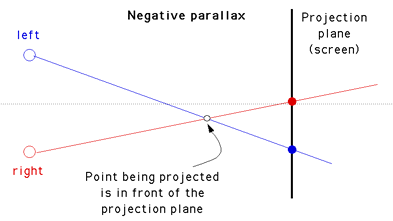
\includegraphics[width=\linewidth, height=3.5cm]{schemas/negative_parallax}
\end{minipage}
\hspace{\fill}
\begin{minipage}[t]{0.32\textwidth}
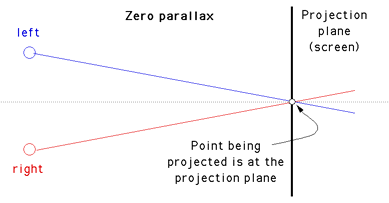
\includegraphics[width=\linewidth, height=3.5cm]{schemas/zero_parallax}
\end{minipage}
\hspace{\fill}
\begin{minipage}[t]{0.32\textwidth}
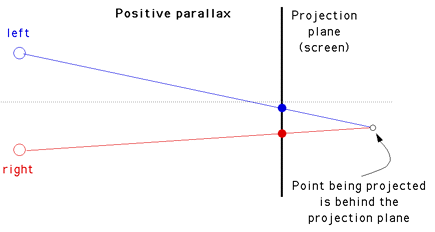
\includegraphics[width=\linewidth, height=3.5cm]{schemas/positive_parallax}
\end{minipage}
\end{subfigure}
\vspace*{-5mm}
\caption{Different parallax situations. Courtesy of Paul Burke's work (source: \href{http://paulbourke.net/stereographics/stereorender/}{paulbourke.net})}
\label{fig:parallax_plane}
\end{figure}

A practical problem with shifting the displayed images on screen is that part of each half-image falls off the boundaries of the screen, therefore losing precious FOV the more we move objects behind the screen. This is also why parallel-type is much used in computer graphics, where it is not a problem to customize virtual camera parameters to cover a higher portion of the scene from the beginning with zero cost.

\begin{figure}
\centering
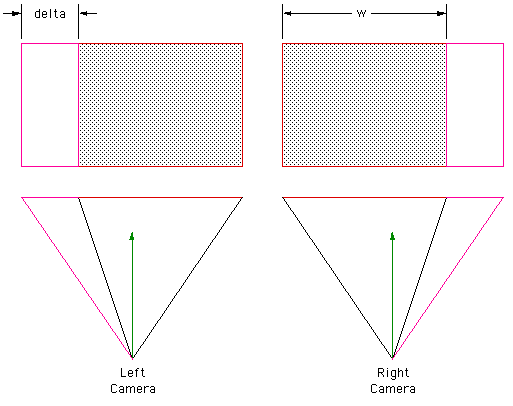
\includegraphics[width=7cm]{schemas/parallel}
\caption{The problem of shifting and losing portion of each image. Paul Burke gives a good formulation of this problem in [N] (source: \href{http://klee.cittastudi.di.unimi.it/~dan/PGL/doc/articoli&libri/CalculatingStereoPairs.pdf} {Creating correct stereo pairs from any raytracer})}
\label{fig:parallel_cameras}
\end{figure}

Also, having most of the scene behind the display is preferred situation in stereoscopy. Having much of the scene too far from the zero-parallax plane causes a disruption of the natural synergy between vergence and accomodation for most users (since objects are not where each eye focuses on). Different reasons make behind-the-screen philosofy a preference: something coming out from the screen more likely will cross its boundaries and will screw up occlusion perception; targets far away are more likely to be on focus toghether with the screen than closer ones.

\subsubsection{Off-axis cameras}
A real camera can be hacked so that it gets all advantages and simplicity of parallel-type configuration without giving away FOV. Instead of shifting display frame afterwards or translating cameras taking the risk of unnatural results, we can play with sensor/lens alignment. By shifting the sensor in respect to the lens, we can decide the actual convergence angle exploiting all available sensor area. What happens is that camera frustrum is no longer symmetric and allows us to cover different areas of the scene without rotating the lens/sensor. This method is also called shifted-lens or skewed-frustrum stereo and is the ideal way of capturing/reproducing stereo pairs [18,19].

\begin{figure}
\centering
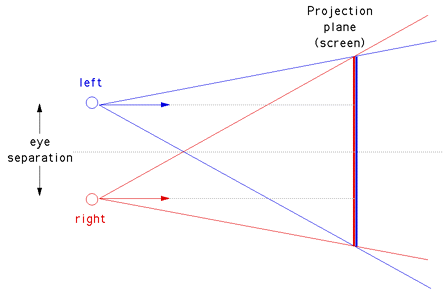
\includegraphics[width=7cm]{schemas/offaxis}
\caption{The image shift is no longer necessary if the view frustrum is shifted by the needed amount}
\label{fig:offaxis_cameras}
\end{figure}

Unfortunately, such vision systems are not very diffused and are difficult to realize in practice due to the high precision needed. Moreover, vergence angle is something to be decided in advance, leaving each device tied to a specific scene and screen target. This is why existing systems of this kind provide adjustable lens/sensor shift and are much more expensive and therefore uncommon.\\
While this effect is hard to achieve in practice, it can be expressed by the pin-hole model (by means of Principal Point Offset position, not centred). However, in 3D graphics world (where cameras could be entirely customized) still many applications don't go beyond the standard virtual camera model, which as we will see is described by focus point, view and up vector and FOV. A virtual camera matrix (as we will see in chapter 3, its "projection" component) is determined by those parameters even though it is possible to entirely customize it to get the desired frustrum.

\subsubsection{Toed-in cameras}
Optical axis in toed-in configuration converge and baseline intersects with the two camera projection planes (epipolar lines are no longer parallel, but their orientation depend on the stereo pair). As we introduced the convergence problem in parallel-type configuration, we mentioned that rotation of the sensor is a way to go. In reality, this is the pursued option in most cases for image capture [19]; the reason is its low-cost implementation, plus a decent approximation of what an off-axis setup would offer.
\begin{figure}
\centering
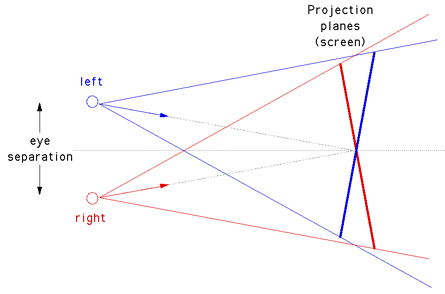
\includegraphics[width=7cm]{schemas/toein}
\caption{Toe-in configuration approximates the off-axis solution by rotating the whole camera body}
\label{fig:toedin_cameras}
\end{figure}
The whole FOV of each camera is indeed preserved and the yaw of each camera can be easily adjusted at capture time. The fundamental problem is that while toe-in stereo makes sense intuitively (as our eyes rotate inwards when we focus on nearby objects), this does not correspond to how 3D is shown. Captured frames are in fact projected into a screen and not differently to each retina. The whole assumption that the image will be displayed on a display orthogonal to viewer's direction (as happens for single camera captures) is still considered valid in 3D movies where there are actually two viewing directions projected into the same plane. This leads to the effect known as "keystoning": artificial vertical disparity is introduced, increasing towards the edges, causing a breakdown of the 3D illusion [15,19]. Even in less severe scenarios where brain is flexible enough to adapt, it will eventually lead to eye strain, not to mention the already present accomodation/convergence conflict. Since this effect is noticeable at the edges, strategies like artificially reduce the amount of eye separation and keep objects, and therefore the viewer's eyes, in the center of the screen may address the symptoms but not the cause.

\begin{figure}
\centering
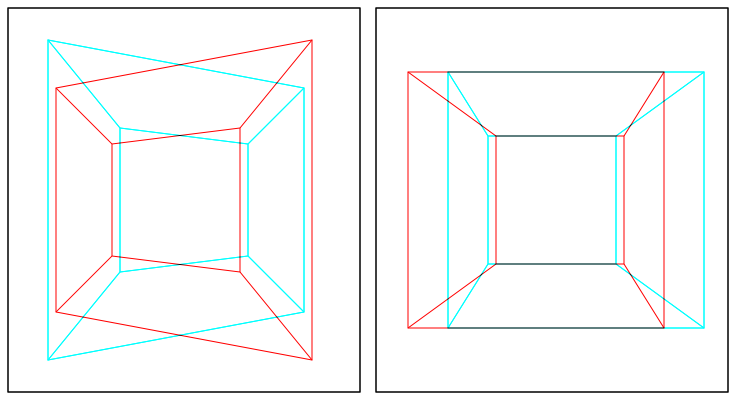
\includegraphics[width=10cm]{pictures/keystoning}
\caption{A 3D cube displayed in toe-in stereo and off-axis stereo (source: \href{http://doc-ok.org/?p=77} {doc-ok.org})}
\label{fig:keystoning}
\end{figure}

Note that this setup is still acceptable for stereo computer vision, which does not really focus about getting acceptable stereopsis and convergence but simply working with as much stereo pairs as possible [20] (how pairs are mapped into depth information is only a matter of calibration). This is also the preferred setup for stereoscopic imaging in photography (where the subject is captured only once and under controlled circumstances) and is still acceptable for video capturing under the assumption that eyes will be most of the time focused on the center of the screen and a good compromise between camera tilt and distance from subject is reached [21].

\subsection{Stereo camera calibration for stereo vision}
Analyzed stereo rig models assume geometric constraints are respected, which is an ideal case. Though human eye can still tolerate slight alignment approximation, stereo computer vision requires precision to obtain reliable data. Stereo calibration process is similar to single camera calibration: it involves more steps, includes getting both intrinsic parameters from each camera and extrinsics for the stereo setup [22]. Camera position and pose are considered in the equation. The aim is to make corresponding epipolar lines in image pairs be parallel to horizontal direction. We won't analyze all proposed solutions to this problem as this falls beyond the scope of this text. We will however put some effort in considering its relationship with previously mentioned configurations. In order to avoid heavy computation in image undistortion, a recent study [23] exploits the relationship between the general-type unconstrainted configuration (which is the non-calibrated rig) to its virtual parallel-type equivalent. It is worth mentioning the proposed algorithm avoids completely complex calculations based on epipolar lines or fundamental matrix. The resulting images appear to be considered as if they were captured by a parallel stereo camera rig with its own optical axis sharing the same origin: raw frame points are re-projected into a new plane and after rectification there is no residue of keystoning, at the cost of reducing percieved FOV. However, since original capture is issued by a toed-in configuration, it cannot be considered a real parallel equivalent; only a portion of rectified frame will contain informational content, leaving black areas whithin view angles reached by the parallel configuration only.

\begin{figure}
\centering

\begin{subfigure} 
\centering   
\begin{minipage}[t]{0.49\textwidth}
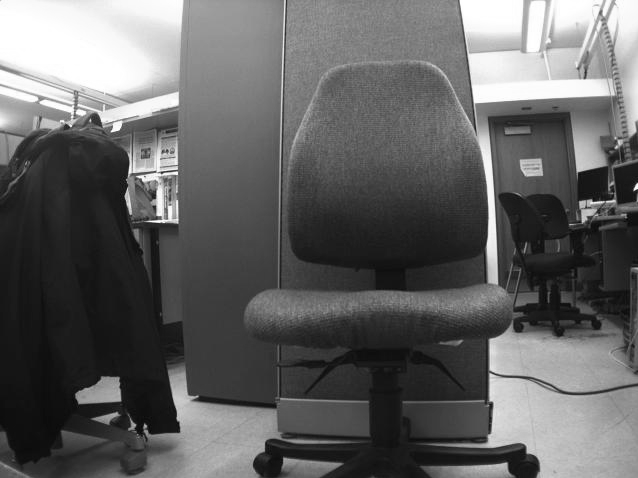
\includegraphics[width=\linewidth, height=5.5cm]{pictures/mono-distorted}
\end{minipage}
%\hspace{\fill}
\begin{minipage}[t]{0.49\textwidth}
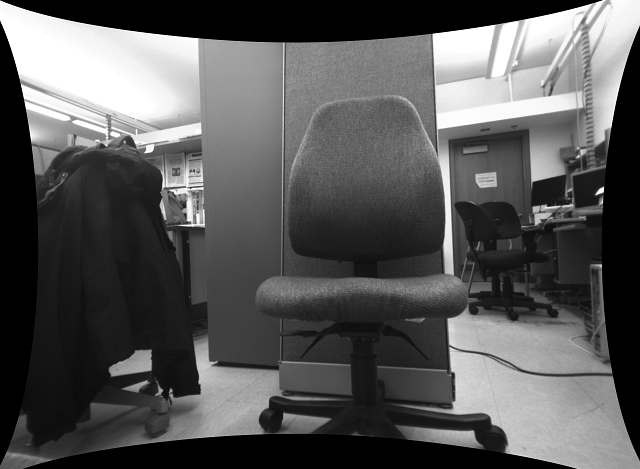
\includegraphics[width=\linewidth, height=5.5cm]{pictures/mono-undistorted}
\end{minipage}
\end{subfigure}
%\vspace*{2mm}
\caption{Image undistortion on a mono calibrated camera image. The pincushion will be centered in the real main focal point.  (source: \href{http://paulbourke.net/stereographics/stereorender/}{paulbourke.net})}
\label{fig:mono_undistort}

\vspace*{0.4cm}

\begin{subfigure}
\centering
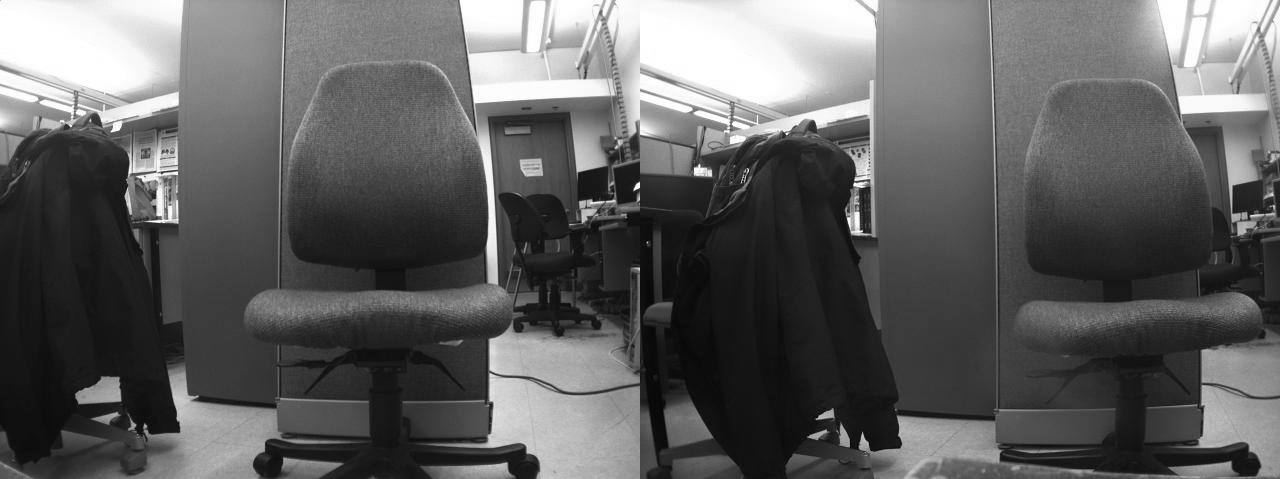
\includegraphics[width=\linewidth]{pictures/stereo-distorted}
%\vspace*{0.4cm} % (or whatever vertical separation you prefer)
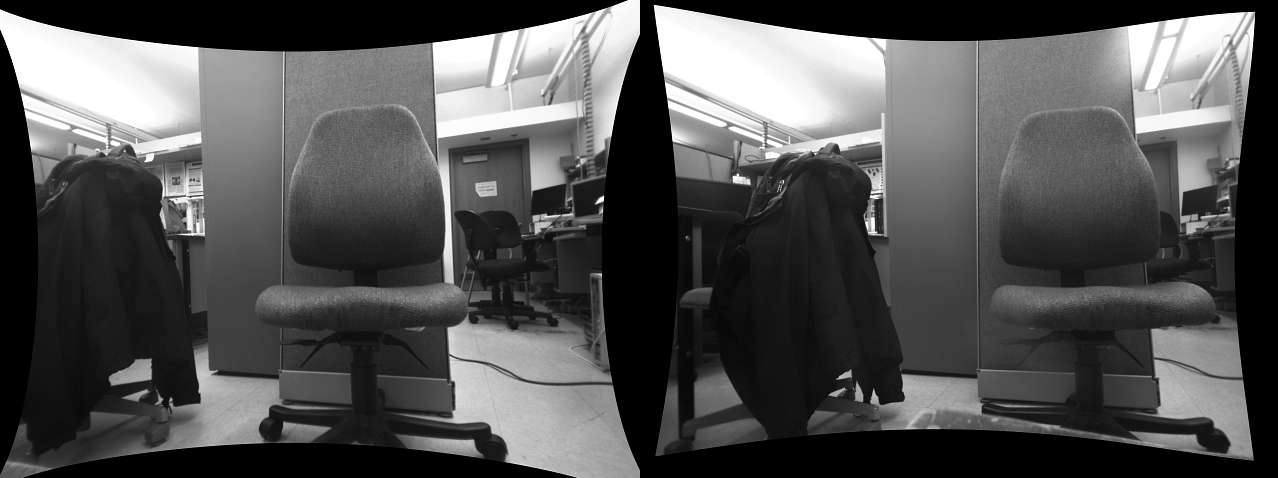
\includegraphics[width=\linewidth]{pictures/stereo-undistorted}
%\vspace*{-6mm}
\caption{Image undistortion on a stereo calibrated camera rig. Note how the two pincushions are also rescaled, rotated or translated relatively so that stereo pairs fall on horizontal lines. (source: \href{http://www.cs.unc.edu/~azuma/ARpresence.pdf}{A Survey of Augmented Reality}). At bottom two respective examples, WorldViz VideoVision powered HMD (left) and Simeye XL100A (right).}
\label{fig:stereo_undistort}
\end{subfigure}

\end{figure}

Stereo calibration is really necessary only where we do not have reasonable control on stereo rig build quality. It is however mandatory for stereo vision algorithms to work properly, which sure is one of the first steps to take to push this work further. Keep in mind that real-time re-sampling of the image is not always feasible and performance is vital to achieve needed FPS. Also consider that effort in getting physical camera alignment right is never too much: FOV is precious and could considerably deteriorate both object detection and user experience [8].

\subsection{From standard to fish-eye stereo}
A classical tool used in computer vision to capture for acquiring images with large FOV are fish-eye optics. Such lenses can work with a standard CCD or CMOS sensors and remove the need of complex mirror or multiple cameras at the cost of high distortion introduced. The undistortion phase is always necessary even for only displaying image to the user. Since achieving wide FOV falls in our goals, we will also count fish-eye stereo as an option. The challenge to integrate fish-eye projection models into a framework for binocular vision with fish-eye lenses has been previously faced [? Fisheye stereo calibration and epipolar rectification], but this regards computer vision only since method is meant to expose the resulting 2D rectified images to automated analysis; in our work we focus also on how to display such images on a non-ordinary display dedicated to immersive applications and how VR, with the results of mono or stereo computer vision, can interact with it.

\section{Modelling first person view in VR}

The stereo oriented approaches presented so far inspired early in the years fields like photography and cinematography, but also later on computer graphics. Virtual reality (VR) is a branch focusing on immersivity, about which we provide an overview of the so called first-person-view (FPV) which aims to reproduce for a user the feel of being (body and mind) in a virtual environment in first person. The reader will agree that FPV modelling is a direct application of what learned so far, under the assumptions . We won't fail to remember  the relevant limitations of simulating a virtual environment and current strategies on how are faced on HMD devices.

\subsection{Head model: IPD and ETN parameters}
Given a 3D virtual environment, stereo in computer graphics can obtained by rendering the same scene from two different view points, much like we do with two cameras in reality. All previously discussed setups can be experimented virtually by implementing custom virtual camera matrices and orienting them in space to achieve desiderd binocularity and convergence. The zero-parallax plane will as well be virtual and can placed in front or behind the real screen. Ideally, how virtual camera should be positioned depends on the display device used and user's distance from it; but over 3D static photography or video footage, a 3D graphics application has a major advantages: applications can assume a initial typical expected case and implement it plus offer options to calibrate the virtual setup, since images are generated at runtime through the virtual cameras. As for user eye convergence, with the support for an eye tracking solution (such as ?tobi), it is possible to adjust virtual orientation dynamically so that correct vergence can be triggered depending on the target object and no precautions must be taken by creator in that sense.

For a video HMD, display is much closer to the eyes and for that to be on focus and to cover human FOV correctly, much more complex optics is involved. Each HMD presents its own implementation of the problem, beginning from user's eye offset up to how virtual camera parameters should be set. Our experiment for instance will be based on a specific HMD set, Oculus Rift Development Kit 2 (DK2), which features wide FOV stereoscopic rendering with suboptimal solution for correct view distortion [? http://doc-ok.org/?p=756]. The current work however strives to separate all elements for stereo graphic rendering from the actual display distortion needed.

\begin{figure}
\centering
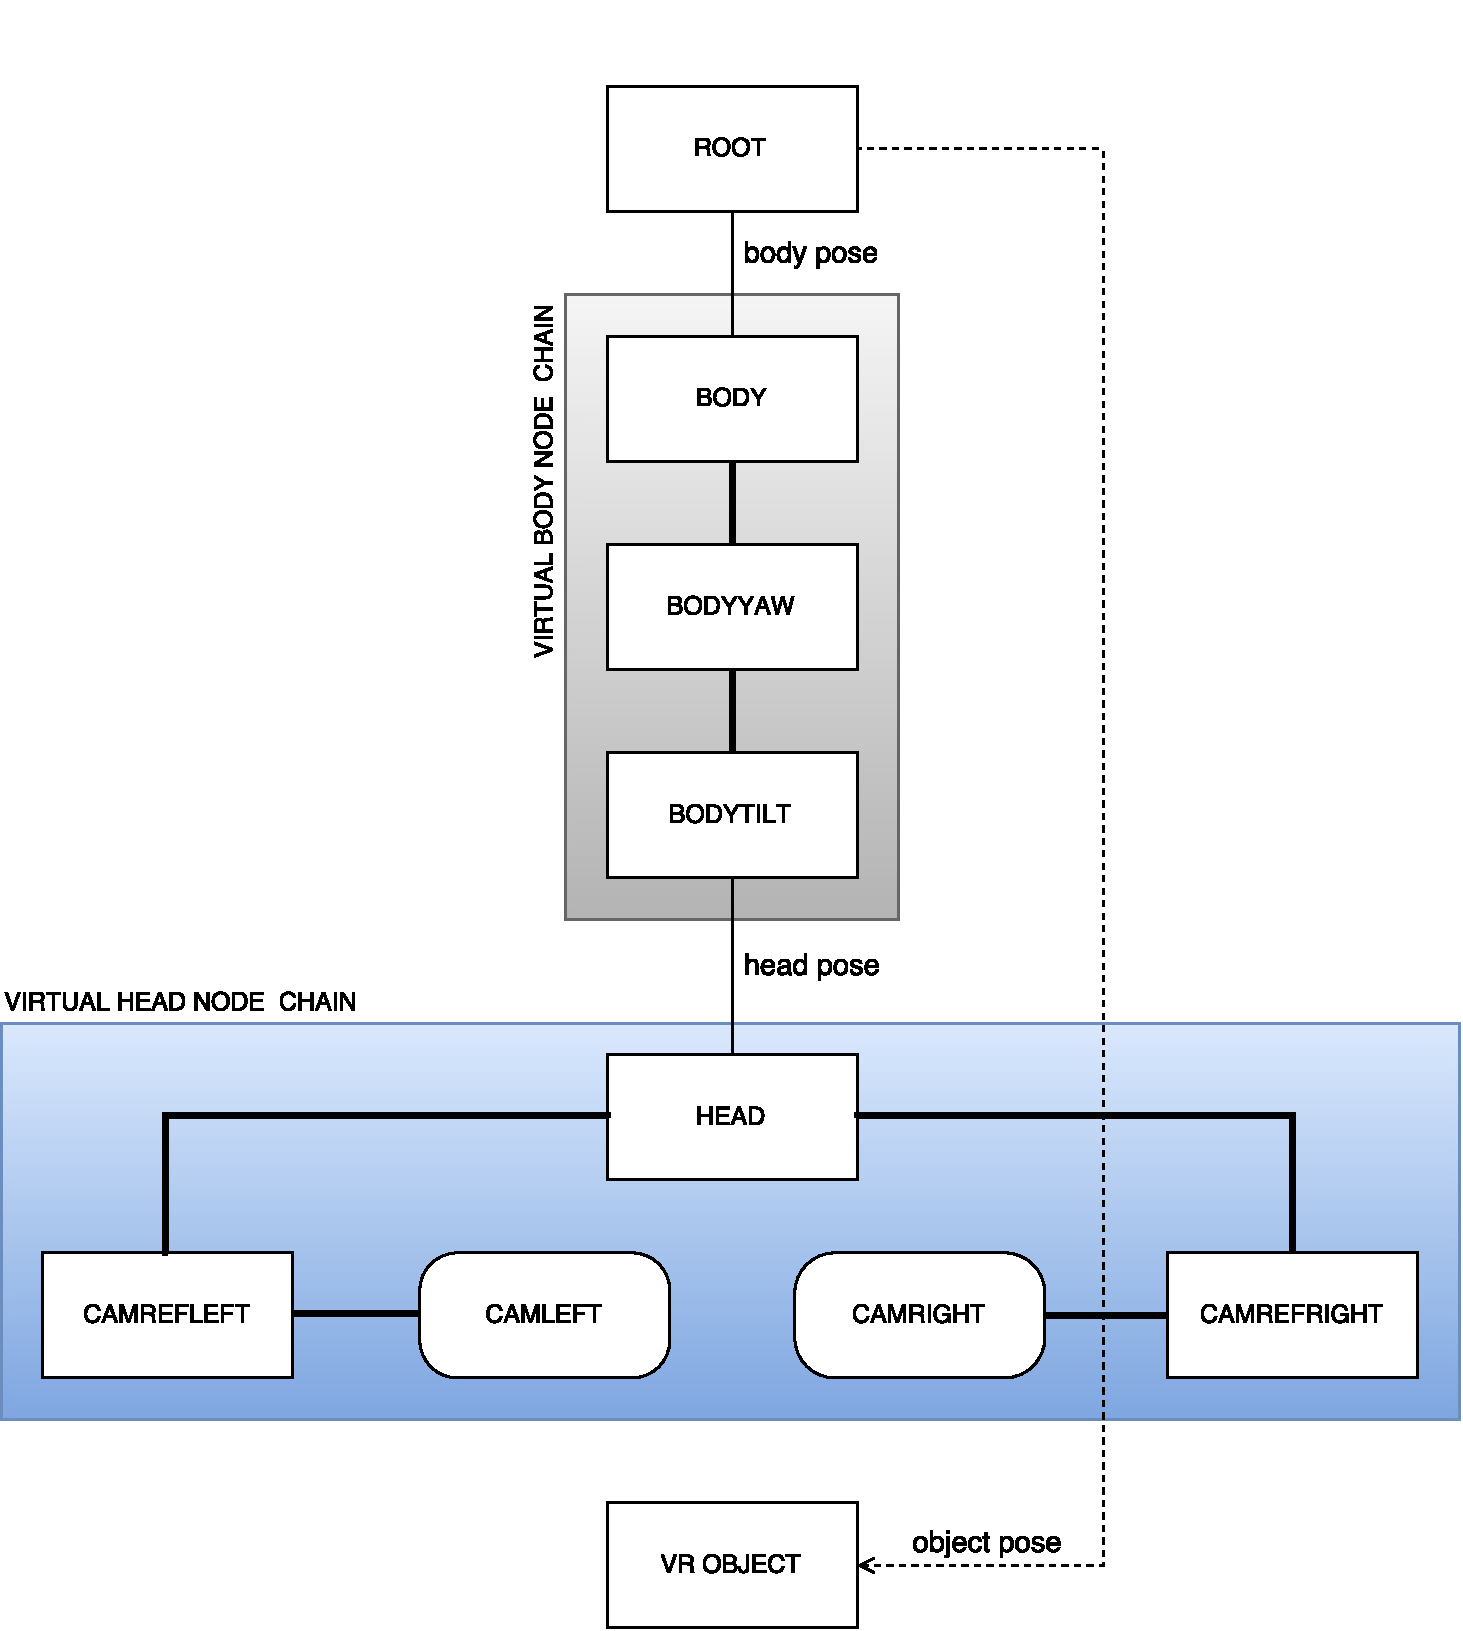
\includegraphics[width=\linewidth]{schemas/classic-head-model_nodetree}
\caption{Thick links indicate nodes with constant position/orientation (for example, IPD and ETN measures) while thinner ones are constantly altered (head pose); body has also been included in the schema for completion, even though body/avatar movements are controlled intependently by other means (body tracking or simple controller).}
\label{fig:classic_head_model}
\end{figure}

Given a head-tracked HMD and a stereo graphics application providing a first-person perspective, real and virtual head of the user correspond: each virtual camera will provide point of view for each eye, while their pose in space will be determined by user's head orientation. To get occlusion and parallax cues perfectly coherent to the movements of a real head, virtual inter-camera distance should match real user inter-pupillary distance (IPD): such measure, as also Oculus Rift documentation suggests, must be manually set, toghether with the actual distance from the eye and neck orbiting point called eye-to-neck distance (ETN). Using a node tree to represent each entity in terms of 3D relative transformation, head model for a first-person perspective VR application appears as in figure N. Camera objects in the schema contain intrinsic parameters defined by HMD requirements: for instance, Oliver Kreylos [?] confirms Oculus Rift provides specific OpenGL camera parameters to implement off-axis stereo, even though official documentation for the version used of the SDK denies it.

\subsection{Low latency rendering and timewarping}
The schema in figure N displays only how, for a head pose, a 3D scene can be rendered correctly prior to further specific HMD-dependent elaboration of HMD. In practice, the system "sensor-renderer-display" is not instantaneous and each step makes a digital system unto itself, meaning different buffering and filtering phases are involved.\\
The following work will not focus specifically on head tracking sensors latency issues (dependent from hardware HMD implementation) but will consider more general countermeasures in terms of overall latency, from the time of sensing to video output.\\
On this behalf, the render-display step do require deeper investigation, since recently classic processing model for 3D graphics applications underwent major optimizations for VR in the last couple of years on this matter. Of particular interest and inspiration for this project are "predictive tracking" and "timewarping", which we will briefly describe.\\
Predictive tracking methods are a very common mitigation technique for reducing latency between a motion sensor capture and its effect on a displayed scene in VR/AR research [12,13,14?]. Although mathematical methods implied are not recent, they are still very used and improve their performance over time due to improvements in sensing and graphics hardware: recent implementations report very fast and accurate measurements that use low-cost sensors deployed in large variety of virtual reality headsets (from 100 to 30-50ms)[? Head Tracking for the Oculus Rift]. What happens is that, given a delta interval in time that can be fixed or dynamically adjusted, a predicting algorithm assumes a physical cinematic quantity to remain constant over that time in the future and computes from it all derived quantities, such as position and velocity if acceleration is chosen. Error in prediction will obviously increase with longer time intervals, but the time interval itself can be reduced when head motion less fast. By setting time end interval to the extimated time of measure evaluation, latency can be mitigated.\\
The cited 50ms wall is hard to beat, since render-display latency comes in play, and the ideal "immersive" latency threshold impossible to hit, documented to be 20ms or below [M. Abrash, "Latency: the sine qua non of AR and VR," Dec. 2012. [Online]. Available: http://blogs.valvesoftware.com/abrash/latency-the-sine-qua-non-of-ar-and-vr]. Even though a sensor measure can be evaluated instantly, the moment it is used in the 3D scene to be rendered, even as a last operation, is still far away from the time of actual display; in other words, there is always a noticeable amount of time between render has started and user sees it.

\begin{figure}
\centering
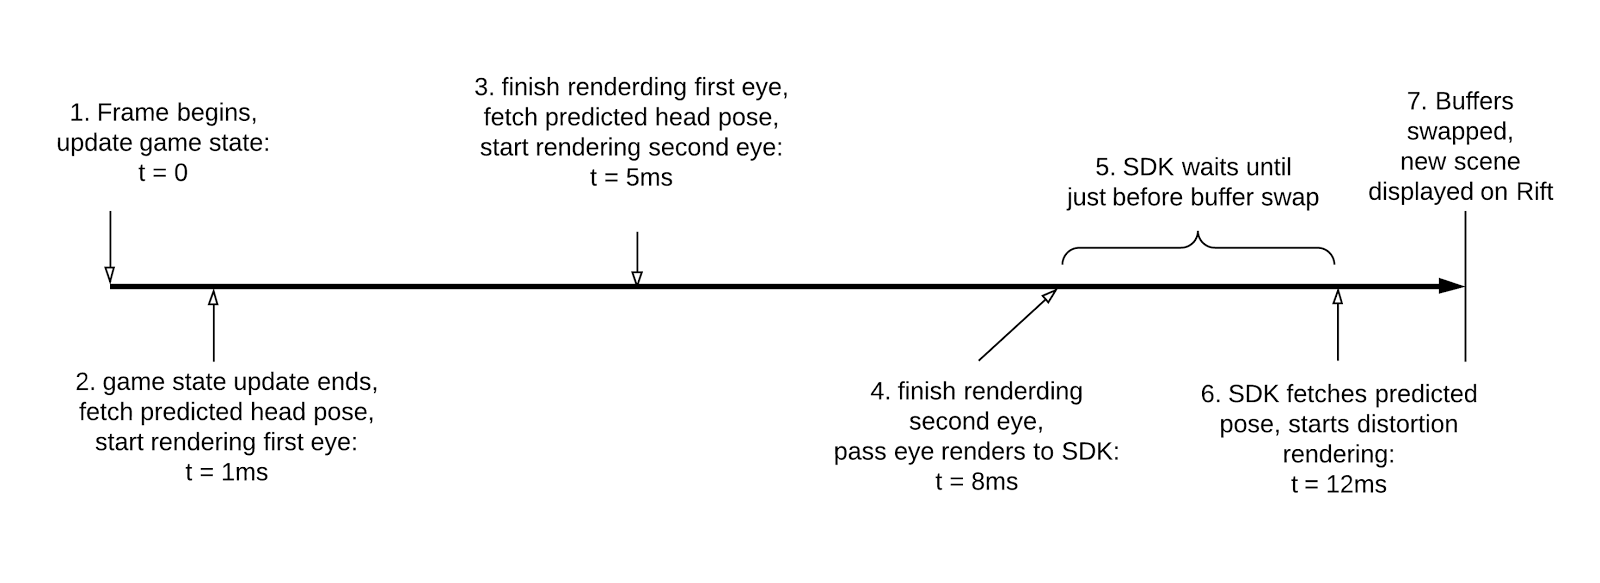
\includegraphics[width=\linewidth]{schemas/timewarp-timeline}
\caption{Render timeline for one frame using pose prediction and asynchronous timewarping. We refer to "SDK" as the part of application that implements those algorithms, not the render pipeline itself. (source: \href{http://rifty-business.blogspot.se/2014/08/using-timewarp-on-oculus-rift.html}{rifty-business.blogspot.se})}
\label{fig:timewarp_timeline}
\end{figure}

According to John Carmack [?], moving sensor evaluation up to render phase would have no effect unless hardware is capable to account for that. In its work, he proposes "timewarping" as a state-of-the-art strategy fit for head-tracked HMD to minimize latency perception: by late evaluation of the sensors, one is able to transform and reproject the 2D render result prior to display on screen and fictionally reproduce an movement of the head in the 3D environment. The expected display time (not render) is then fed to the pose prediction algorithm multiple times: the first two measures are set before starting render of each eye and a final third to evaulate the necessary delta transformation to apply each result (schema N). The timewarping transformation cannot produce correct results in terms of occlusion (since it does not correspond to a real rotation of the head model) and also shows its limits at the edges of the render, since culling has already been performed by rendering (example N), but the reported effectiveness in perception is guaranteed by the high frame/refresh rate of the application/HMD, which updates the view before those issues become relevant for user experience.\\
The implementation of hereby discussed techniques will be taken for granted in our demo application (partial effort is needed with Rift and Oculus SDK) but their results will be discussed and rethinked for immersive AR in chapter 3.

\begin{figure} 
\centering   
\begin{minipage}[t]{0.49\textwidth}
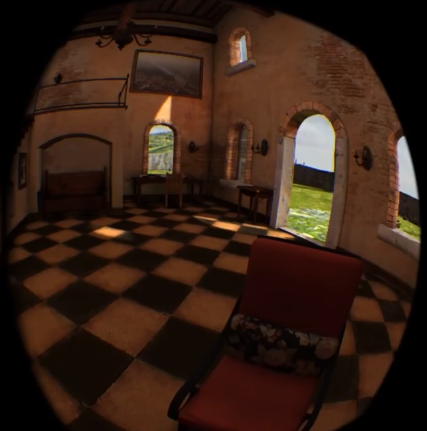
\includegraphics[width=\linewidth, height=7.4cm]{pictures/non-timewarped-chair}
\end{minipage}
%\hspace{\fill}
\begin{minipage}[t]{0.49\textwidth}
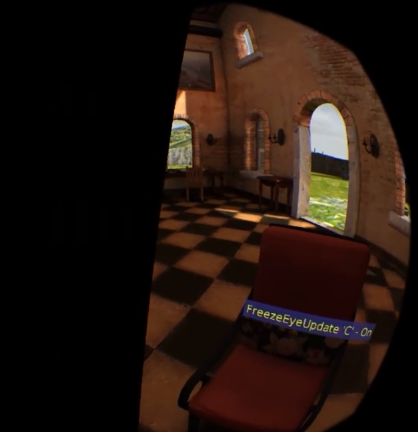
\includegraphics[width=\linewidth, height=7.4cm]{pictures/timewarped-chair}
\end{minipage}
%\vspace*{2mm}
\caption{The rendered result of a head rotation to the left from the chair at standard FPS (left) and at zero FPS (right). At this extreme conditions, timewarping limits can be appreciated. (source: Oculus Tuscany Demo)}
\label{fig:timewarp_example}
\end{figure}

\section{Towards merging real stereo and virtual stereo}

We have seen how to control depth perception with real stereo camera configurations and how it can enhance the simulation of first person view of a virtual scene, which in turn uses virtual model of the real camera. Our next step will be to analyse the relationship between the two and how stereo imagery from virtual and real sources can coexist when both worlds get in contact on a video see-trough HMD device. In the next chapter we will also test the bond and the geometric assumptions made by developing an AR application, while striving to provide feasible solutions to keep the technical and perceptual goals introduced in the first chapter within reach.







